\chapter{文獻探討}
\label{cha:RelatedWork}

本章節針對Free-to-Play類型遊戲興起介紹,並探討關於資料前處理、學習模型選擇、資料不平衡處理以及其評估方式的相關文獻。

\section{Free-to-Play類型遊戲興起}

Free-to-Play(F2P)類型遊戲,是一種玩家無需支付任何費用,即可遊玩該遊戲之大部分內容,與付費型遊戲(買斷制或月費制)形成對比。而在F2P類型遊戲中,針對遊戲商還是可以藉由遊戲內購買(In-App Purchase, IAP)或遊戲內置入廣告方式來賺取營收~\cite{wiki:f2p}。近幾年內,遊戲商皆轉以開發F2P類型遊戲為主,因其類型所帶來之營收,已遠大於付費型遊戲~\cite{lee2018game}。另外,還因為F2P類型遊戲能夠有效的讓玩家流失量降低,透過其無需支付任何費用就能遊玩遊戲的特性,使玩家進入遊戲的門檻大為降低~\cite{10.1007/978-3-030-27355-2_10}。

因此,如何讓玩家於F2P類型遊戲內消費成為了值得探討的議題。近幾年來,許多研究團隊使用機器學習之方式,來進行遊戲領域資料科學方面的研究,大多是以預測玩家是否流失為主~\cite{lee2018game}~\cite{10.1007/978-3-030-27355-2_10}~\cite{lee2016predicting},如表~\ref{tab:MLInGameDataMining}。其中,僅有少數研究團隊進行預測玩家是否會消費之研究~\cite{sifa2015predicting},原因出在於資料之取得困難,可能是礙於遊戲商之營運機密,且遊戲商鮮少與學術研究團隊合作探討此議題~\cite{lee2018game},故投注更多資源於此議題顯得更為重要。
\newpage

\begin{table}[!htb]
	\centering
	\begin{tabular}{|l|l|l|l|l|l|}
		\hline \hline
		\multirow{2}*{Author(s)} & \multicolumn{2}{l|}{Method} & \multicolumn{3}{l|}{Category} \\
    \cline{2-6}
    & Quantitative & Qualitative & \tabincell{l}{Motivation to\\use Game\\Analytics} & \tabincell{l}{CLV\\prediction} & \tabincell{l}{Churn\\prediction} \\
    \hline \hline
    \tabincell{l}{Hadiji et al.\\(2014)} & x &&&& x \\
    \hline
    \tabincell{l}{Runge et al.\\(2014)} & x &&&& x \\
    \hline
    \tabincell{l}{Hanner and\\Zarnekow\\(2015)} & x &&& x & \\
    \hline
    \tabincell{l}{Koskenvoima\\and Mäntimäki\\(2014)} && x & x && \\
    \hline
    \tabincell{l}{Sifa et al.\\(2015)} & x &&& x & \\
    \hline
    \tabincell{l}{Lee et al.\\(2016)} & x &&&& x \\
    \hline
    \tabincell{l}{Perianez et al.\\(2016)} & x &&&& x \\
    \hline
    \tabincell{l}{Voigt and Hinz\\(2016)} & x &&& x & \\
    \hline
    \tabincell{l}{Milosevic et al.\\(2017)} & x &&&& x \\
    \hline
    \tabincell{l}{Demediuk et al.\\(2018)} & x &&&& x \\
    \hline
    \tabincell{l}{Drachen et al.\\(2018)} & x &&& x & \\
    \hline \hline
		\end{tabular}
	\caption[近年來機器學習應用於遊戲領域表]{近年來機器學習應用於遊戲領域表(此表出自~\cite{10.1007/978-3-030-27355-2_10})}
	\label{tab:MLInGameDataMining}
\end{table}
\newpage

\section{資料前處理}

在將巨量資料應用於機器學習前,資料的前處理也是極為重要,相較於在學習模型上進行深入研究與改進,透過資料特徵之轉化及選擇顯得更為重要且有效~\cite{lee2018game}。首先將對資料進行清理,只收集有價值之資料,例如:Tamassia等人只收集遊玩時間超過給定門檻之玩家~\cite{tamassia2016predicting}、Periáñez等人只收集消費金額遠高於一般玩家者~\cite{perianez2016churn}或Runge等人只取付費玩家中前10 \%者~\cite{runge2014churn},上述之清理方式皆只著重於具有高資訊量的資料,而不將無價值的資料放入機器學習中。

而針對資料特徵之探勘,Sifa等人~\cite{sifa2015predicting}將探勘玩家基本資料及玩家行為,再將其進行轉化,例如:取平均值與偏差值於玩家遊玩時間、將玩家國籍分類等等。Lee等人~\cite{lee2016predicting}將探勘玩家行為、玩家購買商品數量、玩家遊戲內交易及玩家遊戲內社交,主要針對玩家於遊戲內的行為軌跡。Martínez等人~\cite{martinez2020machine}將探勘顧客國籍、兩次購買時間差及最後一次購買時間點等等,再將其進行轉化,例如:取平均值、中位數及最大最小值等等,透過數值間的轉化,提升資料集的維度。Hadiji等人~\cite{6932876}將探勘玩家消費商品數量、玩家遊玩天數等等。

\section{學習模型選擇}

在機器學習中,應用於分類預測上為樹狀結構之學習模型最為主流且有效,因其建樹之方式,可以清楚的解釋該筆樣本之預測路徑,進而針對各資料特徵進行重要性的計算與分析~\cite{lee2018game}。另外,在樹狀結構之學習模型中,主流以Bagging及Boosting兩種建樹想法為準:

\begin{itemize}
    \item Bagging為從訓練資料集中,隨機取樣並訓練成多份分類器,而每次訓練資料取出後放回,再抽取,最後之預測結果將由多個分類器投票選出,採多數決,且各分類器間的權重關係皆為相等~\cite{breiman1996bagging},如圖~\ref{fig:Bagging},例如:Random Forest~\cite{breiman2001random}即為Bagging + Decision Tree~\cite{breiman1984classification}。
    \item Bootsing為從訓練資料集中,每次訓練使用相同資料,而第n個分類器於訓練時,將針對第n-1個分類器分類錯誤的資料增大其權重值,以修正分錯的資訊,希望將分錯的資料減少,預測結果將由多個分類器投票選出,各分類器間的權重關係不同,錯誤率越低的分類器,擁有越高的權重~\cite{freund1999short},如圖~\ref{fig:Boosting},例如:Extreme Gradient Boosting~\cite{chen2016xgboost}即為Boosting + Decision Tree。
\end{itemize}
\newpage

\begin{figure}[!htb]
    \begin{center}
      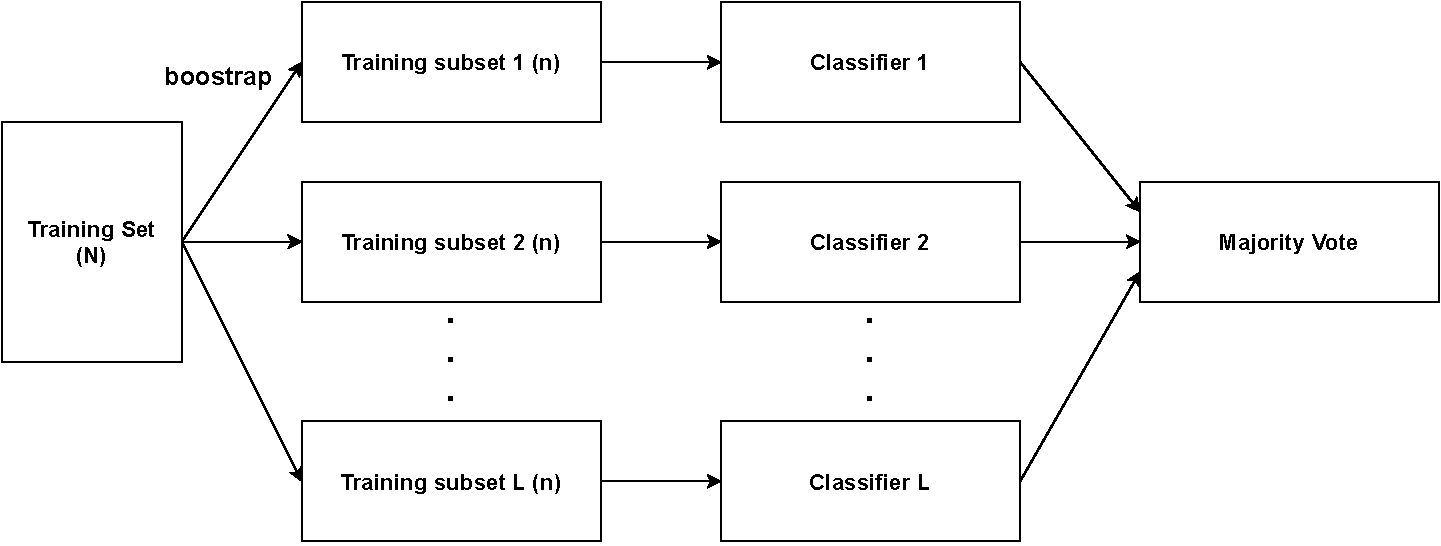
\includegraphics[width=1\textwidth]{figures/Image_Bagging.pdf}
      \caption[Bagging方式建樹示意圖]{Bagging方式建樹示意圖(此圖出自~\cite{tommy2018baggingandboosting})}
      \label{fig:Bagging}
    \end{center}
\end{figure}

\begin{figure}[!htb]
    \begin{center}
      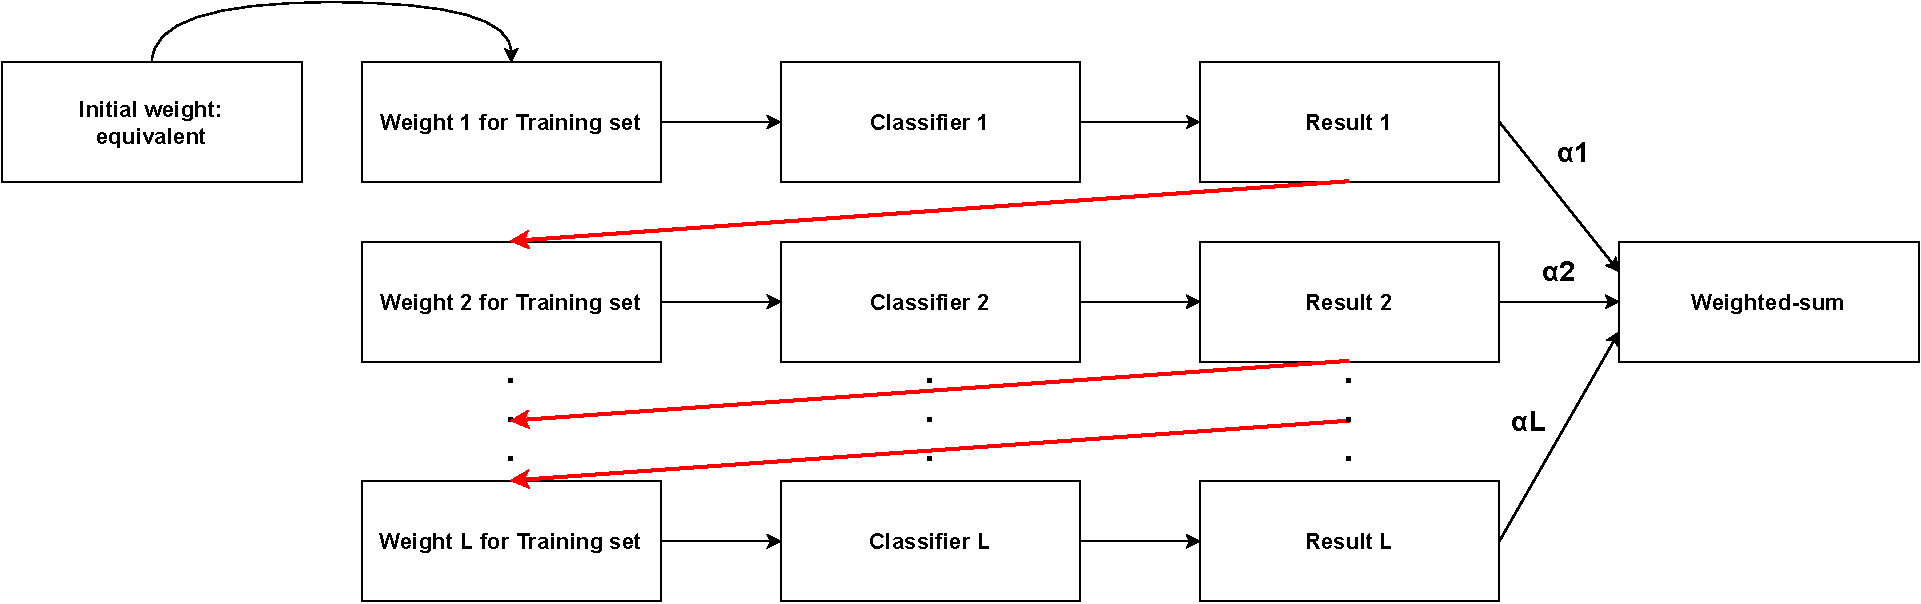
\includegraphics[width=1\textwidth]{figures/Image_Boosting.pdf}
      \caption[Boosting方式建樹示意圖]{Boosting方式建樹示意圖(此圖出自~\cite{tommy2018baggingandboosting})}
      \label{fig:Boosting}
    \end{center}
\end{figure}

Chen與Guestrin~\cite{chen2016xgboost}實作出高效率的Gradient Boosting,稱其為Extreme Gradient Boosting(XGBoost),除了使用Boosting的方式建樹外,還針對錯誤修正的步驟,引入Gradient Descent的概念,加速了學習模型的收斂速度,使其修正錯誤的能力更加精準,大幅減少訓練的時間成本。近年來透過XGBoost來訓練的研究越來越多,且其預測能力皆有不錯的表現~\cite{martinez2020machine}~\cite{semenov2016performance}~\cite{janusz2017helping},明顯優於Bagging建樹方式的其他學習模型。

從上述得知,選用樹狀結構之學習模型將有助於預測分類問題,且其中使用XGBoost之成效最佳。因此,為求本論文之預測付費玩家能夠達到預期,將採用Decision Tree、Random Forest與XGBoost來驗證樹狀結構之優勢以及XGBoost之最佳表現。
\newpage

\section{資料不平衡處理及其評估方式}

在遊戲領域進行機器學習訓練時,往往會遭受到資料不平衡的影響;例如:於預測消費上,非付費玩家將會遠大於付費玩家,導致付費玩家資料過少~\cite{sifa2015predicting}。於預測流失上,流失者將會遠大於非流失者,導致非流失者資料過少~\cite{lee2016predicting},前述研究都採以針對資料集進行處理的方式解決資料不平衡,例如:SMOTE,於少數群添加假資料,使得少數群之樣本數與多數群相等~\cite{chawla2002smote}。本論文因不只預測玩家是否會付費,還需分析玩家之消費原因,故需要透過學習模型產出之預測結果進行分析,如在資料集中填入假資料,將會使得分析失準,無法得到有效的資訊,所以我們將採用在機器學習訓練時,放大少數群之樣本權重值,使得學習模型更加著重於少數群的資訊,如同Boosting方式建樹時,藉由權重值的不同,修正分類錯誤的資訊~\cite{freund1999short}。

在評估資料不平衡資料集時,如果單純計算學習模型之$precision$、$recall$或$F - Score$~\cite{chinchor1993muc},將導致多數群之評估結果壓過少數群之評估結果,使得最終評估失真,無法有效驗證學習模型之成效。因此,在評估不平衡資料時,Sifa等人額外運用$G - Mean$~\cite{kubat1997learning}來評估學習模型之成效~\cite{sifa2015predicting}。藉由上述的概念,本論文將採用$Weighted\ F_{beta} - Score$來評估不平衡資料,使得少數群之評估不被多數群所壓過,使用樣本間的數量權重差來計算多數群與少數群的$F_{beta} - Score$,希望能夠合理的評估學習模型間的表現。